\documentclass[12pt]{report}

\usepackage{amsmath}
\usepackage{pgfplots}
\usepgfplotslibrary{units}
\usepackage[russian]{babel}
\usepackage{filecontents}
\usepackage{titlesec, blindtext, color}
\usepackage{listings}
\usepackage{pdfpages}

\usepackage{titlesec, blindtext, color} 
\definecolor{gray75}{gray}{0.75} 
\newcommand{\hsp}{\hspace{20pt}} 

\usepackage{geometry}
\geometry{top=0.5cm}

%\lstset{ 
%	language=С++,                 
%	basicstyle=\small\sffamily, 
%	numbers=left,              
%	numberstyle=\tiny,        
%	stepnumber=1,              
%	numbersep=5pt,             
%	showspaces=false,          
%	showstringspaces=false,   
%	showtabs=false,             
%	frame=single,            
%	tabsize=2,                
%	captionpos=t,              
%	breaklines=true,           
%	breakatwhitespace=false, 
%	escapeinside={\#*}{*)}   
%}

\lstset{
	language=C++,
	numbers=left,
	frame=single,
	texcl=true,
	basicstyle=\ttfamily
}

\titleformat{\chapter}[hang]{\Huge\bfseries}{\thechapter\hsp\textcolor{gray75}{|}\hsp}{0pt}{\Huge\bfseries}

\begin{document}
	
	
	\begin{titlepage}
		\centering
		{\scshape\LARGE МГТУ им. Баумана \par}
		\vspace{3cm}
		{\scshape\Large Лабораторная работа №6\par}
		\vspace{0.5cm}	
		{\scshape\Large По курсу: "Анализ алгоритмов"\par}
		\vspace{1.5cm}
		{\huge\bfseries Задача коммивояжёра\par}
		\vspace{2cm}
		\Large Работу выполнил: Подвашецкий Дмитрий, ИУ7-54Б\par
		\vspace{0.5cm}
		\LargeПреподаватели:  Волкова Л.Л., Строганов Ю.В.\par
		
		\vfill
		\large \textit {Москва, 2019} \par
	\end{titlepage}
	
	\tableofcontents
	
	\newpage
	\chapter*{Введение}
	\addcontentsline{toc}{chapter}{Введение}
	
	Задача коммивояжёра — одна из самых известных задач комбинаторной оптимизации, заключающаяся в поиске самого выгодного маршрута, проходящего через указанные города хотя бы по одному разу с последующим возвратом в исходный город. В условиях задачи указываются критерий выгодности маршрута (кратчайший, самый дешёвый, совокупный критерий и тому подобное) и соответствующие матрицы расстояний, стоимости и тому подобного. Как правило, указывается, что маршрут должен проходить через каждый город только один раз — в таком случае выбор осуществляется среди гамильтоновых циклов.
	
	Данную задачу можно решить точным методом или же эвристическим. В качестве точного метода будет использован полный перебор, а в качестве эвристического - метод муравьиой колонии.
	
	\textbf{Задачами} данной лабораторной являются:
	\begin{enumerate}
		\item изучение метода полного перебора и метода муравьиной колонии для решения задачи коммивояжёра;
		\item реализация данных двух методов;
		\item экспериментальное подтверждение различий во временнóй эффективности рассматриваемых алгоритмов для различных классов задач;
		\item описание и обоснование полученных результатов в отчете о выполненной лабораторной
		работе, выполненного как расчётно-пояснительная записка к работе.
	\end{enumerate}


	\chapter{Аналитическая часть}
	Задача коммивояжёра относится к классу NP-трудных и не известен алгоритм, который позволет гарантировано её решить за полиномиальное по числу городов N. Однако для небольшого числа городов (N < 15) существует множество способов решения.
	
	В данной лабораторной работе будут исследованы один точный (полный перебо) и один эвристический (муравьиная колония) метод.
	Точные методы позволяют найти наилучший путь, а так же доказать, что найденый путь является таковым.
	В то время как эвристические методы работают существенно быстрее точных, но не гарантируют оптимальности найденого пути.
	
	\textbf{Полный перебор} заключается в перестановки N-1 чисел (при зафиксированном стартовом городе) и поиске пути с минимальной стоимостью (длинной, временем и тд).
	
	\textbf{Метод муравьиной колонии} основан на биологической идеи - принципе существования муравьиной колонии.
	Во время работы данного алгоритма происходит маркировка наиболее удачных путей феромоном.
	
	Работа начинается с размещения муравьёв в вершинах графа (городах), затем начинается движение муравьёв — направление определяется вероятностным методом, на основании формулы вида:

	\begin{displaymath}
		P_{K, ij} = \left\{ \begin{array}{ll}
		\dfrac{(\tau_{ij}^\alpha(t))*(\eta_{ij}^\beta)}{\Sigma(\tau_{iq}^\alpha(t))*(\eta_{iq}^\beta)}
		& \textrm{если он не был в городе i}\\ 
		0 & \textrm{иначе}
		\end{array} \right.
	\end{displaymath}
	
		$\alpha$, $\beta$ - настроечные параметры
		$\alpha$ + $\beta$  = const
		
		$\tau_{ij}$ - кол-во ферамона на ребре ij
		
		$\eta_{ij}$ = 1/{$D_{ij}$}, {$D_{ij}$} - длина (стоимость) ребра ij
		
	После того, как все муравьи закончили поиск, происходит перерасчет ферамонов по формуле:
	\begin{center}
		$\tau_{ij}$(t+1) = $\tau_{ij}$*(1-$\rho$) + $\Sigma$$\Delta$$\tau_{k,ij}$(t)
	\end{center}

	$\rho$ - коэф. рассеивания
	\begin{displaymath}
	\Delta\tau_{k,ij} = \left\{ \begin{array}{ll}
	\dfrac{Q}{L_{k}}
	& \textrm{если ij ребро принадлежит маршруту k-го муравья}\\ 
	0 & \textrm{иначе}
	\end{array} \right.
	\end{displaymath}
	
	Q - нормировачаная константа
	$L_{k}$ - длина пути k-го муравья

	Этот процесс повторяется $T_{max}$ раз.
	\chapter{Конструкторская часть}
	\subsection{Схемы алгоритмов}
	\begin{center}
		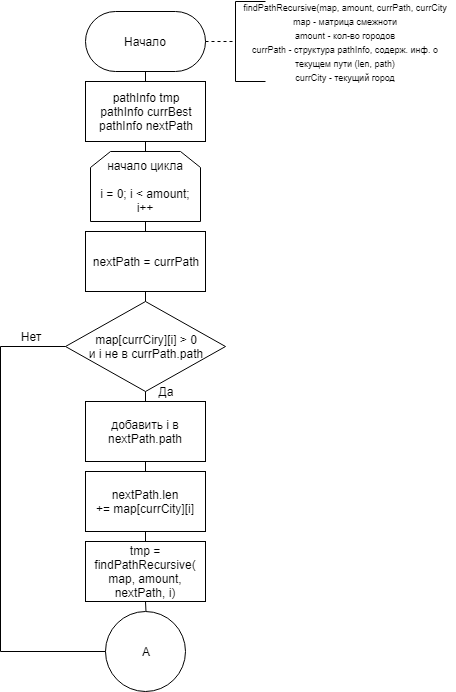
\includegraphics[scale=0.7]{Rec1.png}
		
		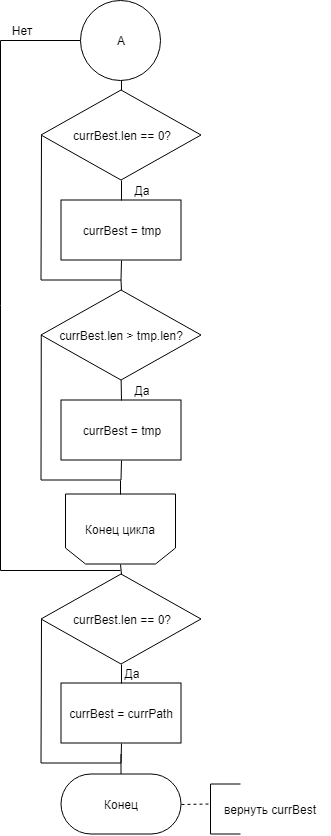
\includegraphics[scale=0.7]{Rec2.png}
		
		Рис. 1. Схема рекурсивной реализации решения задачи коммивояжёра методом полного перебора
	\end{center}
	
	
	
	
	
	
	
	
	
	
	
	
	
	
	
	
	
	
	
	
	
	
	
	
	
	
	
	
	
	
\end{document}